\documentclass[journal]{IEEEtran}
\IEEEoverridecommandlockouts
%%%%%%%%%%%%%%%%%%%%%%%%%%%%%%%%%%%%%%
%%%%%%%% PRINCIPALES PAQUETES %%%%%%%%
%%%%%%%%%%%%%%%%%%%%%%%%%%%%%%%%%%%%%%
\usepackage{fancyhdr}
\usepackage{graphicx}
\usepackage[spanish, es-tabla]{babel}
\usepackage[utf8]{inputenc}
\usepackage{color}
\usepackage{hyperref}
\usepackage{wrapfig}
\usepackage{array}
\usepackage{multirow}
\usepackage{adjustbox}
\usepackage{nccmath}
%\usepackage{anysize}
\usepackage{subfigure}
\usepackage{amsfonts,latexsym} % para tener disponibilidad de diversos simbolos
\usepackage{enumerate}
\usepackage{booktabs}
\usepackage{float}
\usepackage{threeparttable}
\usepackage{array,colortbl}
\usepackage{ifpdf}
\usepackage{rotating}
\usepackage{cite}
\usepackage{stfloats}
\usepackage{url}
\usepackage{listings}
\usepackage{tikz}
\usepackage{hyperref}
\usepackage{multicol}

\definecolor{gray97}{gray}{.97}
%Estilo del código
\lstset{ frame=Ltb,
  framerule=0pt,
  aboveskip=0.5cm,
  framextopmargin=3pt,
  framexbottommargin=3pt,
  framexleftmargin=0.4cm,
  framesep=0pt,
  rulesep=.4pt,
  backgroundcolor=\color{gray97},
  rulesepcolor=\color{black},
  %
  stringstyle=\ttfamily,
  showstringspaces = false,
  basicstyle=\ttfamily,
  commentstyle=\color{blue},
  keywordstyle=\color{red},
  %
  numbers=left,
  numbersep=15pt,
  numberstyle=\ttfamily,
  numberfirstline = false,
  breaklines=true,
}
%%%%%%%%%%%%%%%%%%%%%%%%%%%%%%%%%%%%%%%%%%%
%%% CREAR Y REESCRIBIR ALGUNOS COMANDOS %%%
%%%%%%%%%%%%%%%%%%%%%%%%%%%%%%%%%%%%%%%%%%%
\newcolumntype{P}[1]{>{\centering\arraybackslash}p{#1}}
%% Se crea un nuevo tipo de columna llamada P.
\newcommand{\tabitem}{~~\llap{\textbullet}~~}
\newcommand{\ctt}{\centering\scriptsize\textbf}
%%\ctt abrevia el comando \centering\scriptsize\textbf
\newcommand{\dtt}{\scriptsize\textbf} %%\dtt abrevia el comando \scriptsize\textbf
\renewcommand\IEEEkeywordsname{Palabras clave}

\renewcommand\IEEEkeywordsa{Key words}
\renewcommand\abstracteee{Abstract}

%%%%%%%%%%%%%%%%%%%%%%%%%%%%%%%%%%%%%%%%%%%

\graphicspath{ {Figs/} }  %%Ruta donde se encuentran las imágenes, que esté vacio indica que las imagenes están dentro de la misma carpeta que contiene el archivo .tex

%%%%%%%%%%%%%%%%%%%%%%%%%%%%%%%%%%%%%%%%%%%%%%%%%%%%%%%%%%
%%% ENCABEZADO DE LAS PÁGINAS  %%%%%%%%%%%%%%
%%%%%%%%%%%%%%%%%%%%%%%%%%%%%%%%%%%%%%%%%%%%%%%%%%%%%%%%%%
\newcommand{\MYhead}{\smash{\scriptsize
    \hfil\parbox[t][\height][t]{\textwidth}{\centering
      \begin{picture}(0,0)
        \put(-15,-20){
\includegraphics[width=4CM]{Figs/logo UV.png}} \end{picture}
      \hspace{6.4cm}
      PROYECTO - FÍSICA COMPUTACIONAL II-2022\hspace{5.15cm}
      \, \\
      \hspace{5.2cm} Prof. Karem Rodríguez\hspace{3cm} Enero
      2023\\
      \underline{\hspace{ \textwidth}}}\hfil\hbox{}}}
\makeatletter
% normal pages
\def\ps@headings{%
  \def\@oddhead{\MYhead}%
  \def\@evenhead{\MYhead}}%
% title page
\def\ps@IEEEtitlepagestyle{%
  \def\@oddhead{\MYhead}%
  \def\@evenhead{\MYhead}}%
\makeatother
% make changes take effect
\pagestyle{headings}
% adjust as needed
\addtolength{\footskip}{0\baselineskip}
\addtolength{\textheight}{-1\baselineskip}
%%%%%%%%%%%%%%%%%%%%%%%%%%%%%%%%%%%%%%%%%%%%%%%%%%%%%%%%%%
%%%%%%%%%%%%%%%%%%%%%%%%%%%%%%%%
%%%%% INICIO DEL DOCUMENTO %%%%%
%%%%%%%%%%%%%%%%%%%%%%%%%%%%%%%%
\begin{document}
%%%%%%%%%%%%%%%%%%%%%%%%%%%%
%%% TÍTULO DEL DOCUMENTO %%%
%%%%%%%%%%%%%%%%%%%%%%%%%%%%
\title{IV. PROPAGACIÓN DE ENFERMEDADES}
%%%%%%%%%%%%%%%%%%%%%%%%%%%%
%%%%%%%%% AUTORES %%%%%%%%%
%%%%%%%%%%%%%%%%%%%%%%%%%%%
\author{Andrés Felipe Valencia \\
  \textit{andres.valencia.fonseca@correounivalle.edu.co}\\% stops a space
  \and
  Nicolás Aguilera García \\
  \textit{nicolas.aguilera@correounivalle.edu.co}\\
  \thanks{El presente documento corresponde al articulo final del
    proyecto de Fisica computacional}} %\thanks anexa una nota a pie de página donde se puede colocar alguna información sobre la naturaleza del documento.
%%%%%%%%%%%%%%%%%%%%%%%%%%%

% Comando que indica la generación del título
\maketitle

%%%%%%%%%%%%%%%%%%%%%
%%%%%% RESUMEN %%%%%%
%%%%%%%%%%%%%%%%%%%%%
\begin{abstract}

\end{abstract}
% En el resumen no se recomienda colocar citaciones bibliográficas.

%%%%%%%%%%%%%%%%%%%%%%
%%% PALABRAS CLAVE %%%
%%%%%%%%%%%%%%%%%%%%%%
\begin{IEEEkeywords}

\end{IEEEkeywords}
%%%%%%%%%%%%%%%%%%%%%%
%\IEEEpeerreviewmaketitle

\begin{abstracteee}

\end{abstracteee}
% En el resumen no se recomienda colocar citaciones bibliográficas.

%%%%%%%%%%%%%%%%%%%%%%
%%% PALABRAS CLAVE %%%
%%%%%%%%%%%%%%%%%%%%%%
\begin{IEEEkeywordsa}

\end{IEEEkeywordsa}

%%%%%%%%%%%%%%%%%%%%%%%%%%%%%%%%%%%%%
%%% PRIMERA SECCIÓN DEL DOCUMENTO %%%
%%%%%%%%%%%%%%%%%%%%%%%%%%%%%%%%%%%%%
\section{Introducción}
\IEEEPARstart{E}{l} presente trabajo es el desarrollo numérico, bajo el uso de
lenguaje \textbf{\textit{C++}},
orientado al análisis matemático del modelo epidemiológico Ross \cite{Ross} y
McKendrick \cite{Kermack} a nivel poblacional conocido como modelo
\textbf{\textit{SIR}}.
Es a través de la modelación de procesos biológicos que la epidemiología
teórica recibe su mayor aporte.
Así que se opta por solucionar mediante el método de
\textbf{\textit{Runge-Kutta 4}} el conjunto de ecuaciones acopladas del modelo,
considerando de manera particular las condiciones
iniciales, y los parámetros propios de la enfermedad.

\subsection{Modelo de Kermack y McKendrick}

El estudio fundamental de Kermack \cite{Ross} y McKendrick \cite{Kermack} ha
sido de gran importancia en las últimas décadas. Su modelo
\textbf{\textit{SIR}}, susceptible-infeccioso-recuperado, y sus variaciones,
se han convertido en modelos básicos para sistemas no lineales que son
utilizados no solo por estudiantes interesados en aplicaciones matemáticas en
biología,
sino también para explicar a responsables de políticas, epidemiólogos y
expertos en salud pública la importancia del estudio de dinámica en
enfermedades contagiosas.\newline

Los campos de salud pública y epidemiología han sido dominados, con buenas
razones, por el uso de modelos estadísticos, sin embargo, se espera,
que el uso de modelos dinámicos aporte una nueva perspectiva, ya que permite a
teóricos y prácticos formular nuevas preguntas dentro de un marco que permite
explorar el impacto de intervenciones en la dinámica de transmisión de
enfermedades contagiosas.
Además, los modelos utilizados deben dar cuenta de los mecanismos responsables
de los patrones observados en la transmisión de una enfermedad contagiosa.
Este proceso ayuda a identificar, cuantificar, evaluar e implementar políticas
de intervención dirigidas a reducir el impacto de la epidemia o incluso brotes
pandémicos a través de la reducción del impacto de estos mecanismos.

\subsection{Modelos de Compartimentos}\label{Modelos}
%%%MOTROS ODELOS SI, SIR, SIS, Y SIRS VACUNACIÓN%%%%%%%%%%%
Los modelos compartimentales constituyen una técnica para simplificar la
modelización matemática que describe el flujo de material en sistemas
biológicos \cite{compartimientos}.
Estos modelos, se dividen en un número de compartimentos por los que circula el
material con flujos de entrada y salida. Este modelo
sirve para simular diferentes interacciones, entre ellas una de sus
aplicaciones se da en la epidemiología. Por lo general, un modelo
epidemiológico de compartimientos, se divide en clases y subclases de
individuos, y se estiman tases de transición, para modelar el comportamiento
en base a un sistema de ecuaciones diferenciales.\\
\newline
En particular si la población se clasifica, en susceptibles $S$, infectados $R$
y recuperados $R$, se tienen los siguientes tipos de modelos;
\begin{enumerate}
  \item \textbf{\textit{SI}} la enfermedad del SIDA es un ejemplo que se
        ajusta a este modelo \cite{SIDA}, aunque actualmente se está desarrollando
        modelos mucho mas complejos para tratar esta enfermedad.
  \item \textbf{\textit{SIR}} Sirve para describir enfermedades virales,
        como la rubéola o la sarampión \cite{Rubeola}.
  \item \textbf{\textit{SIS}} Modela el caso en que los individuos
        infectados pueden retornar a la clase susceptible, es decir no adquieren
        inmunidad. El dengue \cite{Dengue} es una enfermedad de este tipo.
  \item \textbf{\textit{SIRS}} Es un modelo con capacidad de soporte,
        esto significa que el número de susceptibles no crece indefinidamente, puede
        modelar la influenza \cite{Influenza}.
  \item \textbf{\textit{SIRS-V}} Recoge los modelos anteriores, y además
        modela la capacidad de vacunación sobre la población \cite{Vacunacion}, siendo
        este modelo uno de los mas completos.
\end{enumerate}

\begin{figure}[H]
  \centering
  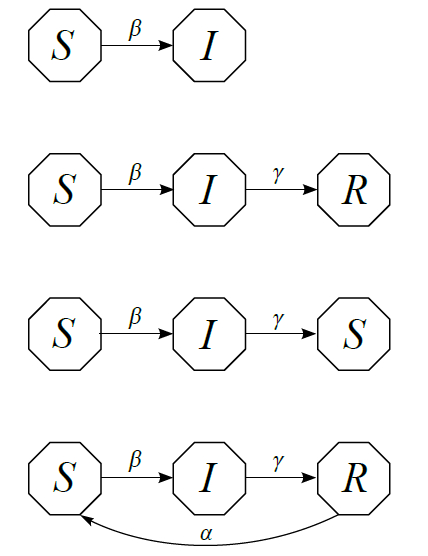
\includegraphics[scale=0.34]{Modelos.png}
  \caption{Modelos tipo SI, SIR, SIS y SIRS de compartimentos}
\end{figure}
%%%%%%%%%%%%%%%%%%%%%%%%%%%%%%%%%%%%%%
%%%MMODELO SIR%%%%%%%%%%%%%
\subsection{Modelo SIR}
Según este modelo \cite{Anderson} los individuos de la población
sobre la cual actúa la enfermedad, que en principio se considera constante, se
clasifican en los siguientes grupos:

\begin{itemize}
  \item \textbf{Susceptibles}, son aquellos individuos sanos pero que en
        potencia se pueden
        enfermar.
  \item \textbf{Infectados}, son los individuos enfermos.
  \item \textbf{Removidos}, son aquellos que se han recuperado, y
        permanecen inmune a la misma sin poder propagarla.
\end{itemize}

Se denota por $S(t)$, $I(t)$ y $R(t)$ el número de individuos susceptibles,
infectados y removidos respectivamente.
En su versión más simple el modelo \textbf{\textit{SIR}} supone la siguiente
retroalimentación $S \rightarrow I \rightarrow R$.\newline

Si consideramos una relación mas simple, que nos da cuenta de la relación entre
cada población con la población total $N$, de este modo;
\begin{equation} \label{poblaciones}
  \begin{split}
    s(t) = \frac{s(t)}{N},\\
    i(t) = \frac{i(t)}{N},\\
    r(t) = \frac{r(t)}{N}\\
  \end{split}
\end{equation}

Para describir entonces la dinámica de la enfermedad se propone el siguiente
sistema:

\begin{equation}\label{SIR}
  \begin{split}
    \frac{ds}{dt} = -bs(t)i(t),\\
    \frac{di}{dt} = bs(t)i(t)-ki(t),\\
    \frac{dr}{dt} = -ki(t)\\
  \end{split}
\end{equation}

Donde $b$ y $k$, son parámetros de la enfermedad, más estrictamente; $k$ es la
tasa de remoción de individuos infectados, quiere decir, una
número de miembros infectados que pasa a la clase de removidos por unidad de
tiempo.\\
Mientras $b$ es la tasa de contacto, representa la capacidad de infectar que
posee la enfermedad. En el modelo que estamos considerando los parámetros
depende de la enfermedad
particular que se estudié, y por lo tanto, puede también depender de factores
sociales y
de comportamiento. En general es difícil estimar ambas constantes.

%%% SUPOSICIONES DEL MODELO%%%%
\subsubsection{Hipótesis}
Este modelo, se sustenta bajo ciertas suposiciones, que limitan la capacidad de
aplicación del mismo, lo que lo convierte en un modelo sencillo,
más sin embargo superar estas suposiciones involucra mejorar el modelo, en la
sección \ref{Modelos} se muestran algunos ejemplos. En el caso del modelo
\textbf{\textit{SIR}} \ref{SIR}
sobre el que se trabaja, se parte bajo los siguientes supuestos;

\begin{enumerate}
  \item  El tamaño de la población $N$ es constante, es decir no se
        consideran muertes, ni se tiene en cuenta los nacimientos dentro de la
        población
        durante la epidemia, esto implica la relación;
        \begin{equation*}
          \frac{d(s+i+r)}{dt} = 0
        \end{equation*}
        Esta hipótesis se consigue de manera razonable en epidemias de
        corta duración.
  \item La enfermedad únicamente se propaga, bajo la ley de acción de
        masas entre la población de susceptibles e infectados, como
        tambien se supone que la transmisión se rige por la incidencia
        común, entre las mismas poblaciones, lo que se refleja en el parámetro
        $b$, una taza constante de contagios que es proporcional al
        numero de contactos entre los individuos susceptibles e infectados.
  \item La taza de recuperación de individuos infectados $k$, no varia
        bajo la dinámica de las poblaciones ni de la enfermedad, es decir es una
        constante.
\end{enumerate}

\section{Metodología}
%%%%ESTABLECER METOOD DE SOLUCIÓN, CONDICIONES INICIALES, Y PARAMETROS%%%%%%%%%%%%%%%
La matemática ha sido una herramienta que ha generado un gran avance dentro de
cada una de las
disciplinas de la biología moderna, acompañada de la estadística y la
computación. El propósito de este trabajo
es solucionar el problema de los modelos epidemiológicos, y simular el
comportamiento de las poblaciones, bajo
circunstancias establecidas, para llevarlo a cabo, se busca implementar
computacionalmente métodos de soluciones numéricas.\\

El conjunto de ecuaciones diferenciales acopladas \ref{SIR}, se convierte un
problema de alto nivel analítico,
no obstante existen desarrollos que tratan las soluciones de ese tipo de
modelos, dando soluciones algebraicas \cite{Sulucion_analitica}.
Sin embargo el desarrollo de la computación ha permitido implementar de manera
mas eficiente técnicas o métodos
para solucionar numéricamente ecuaciones diferenciales, en particular en este
articulo se opta por utilizar el método \textbf{\textit{Runge-Kutta}} de orden
$4$.
Como se mencionó en la introducción, el código se realiza en
\textbf{\textit{C++}}, el repositorio completo se puede encontrar en
\emph{GitHub} \cite{GitHub}
[ver
  \href{https://github.com/niaggar/propagacion-de-enfermedades-project.git}{Propagacion
    de enfermedades}].

\subsection{Runge-Kutta 4 para ecuaciones acopladas}
Los métodos de Runge-Kutta son un conjunto de métodos genéricos iterativos,
explícitos e implícitos, de resolución numérica de ecuaciones diferenciales
\cite{Runge-kutta},
existen variantes de este método que permiten mejorar la aproximación de la
solución, en general dependen del orden del método, este es el numero de pasos
entre cada $\Delta t$.\\

El problema principal a resolver es la ejecución del método para la solución de
un sistema de $3$ ecuaciones
diferenciales acopladas. En primer lugar se definen las ecuaciones que definen
el modelo \ref{SIR}, y el primer
obstáculo que se presenta es como aplicar el método a un sistema de ecuaciones
acopladas, para ello se definen $3$ conjuntos
cada uno con $4$ coeficientes $k_{i, j}$ como términos de aproximación
intermedios, y se plantea el método \textbf{RK},
naturalmente siguiendo la idea de concatenación de cada conjunto de
coeficientes. Para conseguir más eficacia al momento
de extrapolar este código para el desarrollo de otros modelos, se define como
una \textit{Clase}, que recibe como parámetro
el modelo a implementar.

\subsection{Valores iniciales y parámetros}
%%%%VALORES INICIAALES&&&&&&&&&&&&&&&
Para la ejecución de la simulación es necesario un problema de valor inicial,
así que se escribe un comando que permita
introducir por consola, los valores iniciales, que corresponde al numero
inicial de individuos de cada población dentro del modelo. De forma arbitraria
se toma para este desarrollo y a manera de análisis una población total $N=7,900,000$, y
los siguientes valores iniciales;
\begin{equation}
  \begin{split}
    S(0) = 7,900,000,\\
    I(0) = 10,\\
    R(0) = 0\\
  \end{split}
\end{equation}

Pero dado que se usara la relación \ref{poblaciones}, estas condiciones iniciales corresponden a;
\begin{equation}
  \begin{split}
    s(0) = 1,\\
    i(0) = 1, 27 \times 10^{-6},\\
    r(0) = 0\\
  \end{split}
\end{equation}


%%%%PARAMETROS%%%%%%%%%%%%%


%%%%%%%%%%%%%%%%%%%%%%%%%%%%%%%%%%%%%%%%%%%%%%
%%%%%% SECCIONES DE DISEÑO Y DESARROLLO %%%%%%
%%%%%%%%%%%%%%%%%%%%%%%%%%%%%%%%%%%%%%%%%%%%%%
\section{Solución propuesta}

\section{Simulaciones y pruebas}
\emph{testbench} o pruebas realizadas

\section{Implementación de la solución}

%%%%%%%%%%%%%%%%%%%%%%%%%%%%%%%%%%%%%%%%%
%%%%%%%%%%% SECCIONES FINALES %%%%%%%%%%% 
%%%%%%%%%%%%%%%%%%%%%%%%%%%%%%%%%%%%%%%%%
\section{Resultados}

%%%%%%%%%%%%%%%%%%%%%%%%%%%
%%%%%%%%%%%%%%%%%%%%%%%%%%%%%%%%%%%%%
%%%%%%%%%%%% CONCLUSIONES %%%%%%%%%%%
%%%%%%%%%%%%%%%%%%%%%%%%%%%%%%%%%%%%%
\section{Conclusiones}

%%%%%%%%%%%%%%%%%%%%%%%%%%%%%%%%%%%%%

\ifCLASSOPTIONcaptionsoff
  \newpage
\fi

%%%%%%%%%%%%%%%%%%%%%%%%%%
%%%%%% BIBLIOGRAFIA %%%%%%
%%%%%%%%%%%%%%%%%%%%%%%%%%
\begin{thebibliography}{1}

  \bibitem{Ross}
  Ross R.. The prevention of malaria (2nd edition, with Addendum). John
  Murray, London. 1911.
  \bibitem{Kermack}
  Kermack, W. O. and McKendrick, A. G. . A Contribution to the
  Mathematical Theory of Epidemics
  Royal Society of London Proceedings Series A. 1927;115:700–721.
  \bibitem{compartimientos}
  Driessche P. Wu J. (Eds.). Mathematical Epidemiology (Lecture Notes in
  Mathematics / Mathematical
  Biosciences Subseries). Springer 2008
  \bibitem{SIDA}
  Driessche P. Wu J. (Eds.). Mathematical Epidemiology (Lecture Notes in
  Mathematics / Mathematical
  Biosciences Subseries). Springer 2008.
  \bibitem{Rubeola}
  Brauer, F. and Castillo-Chávez, C. . Mathematical Models in Population
  Biology and Epidemiology.
  Springer, New York 2012.
  \bibitem{Dengue}
  Esteva L. Vargas C.. Analysis of a dengue disease transmission model.
  Mathemtical Biosciences.
  1998;150:131–151.
  \bibitem{Influenza}
  Pava E. De. Modelado Matemático de la transmisión de gripe AH1N1.
  Matemáticas Enseanza
  Universitaria.. 2010;XVIII:1–10.
  \bibitem{Vacunacion}
  Hernández, M. E. (2021). Vacunación óptima para un modelo SIRS. Revista
  De Educación Matemática, 29(2).
  Recuperado a partir de
  \url{https://revistas.unc.edu.ar/index.php/REM/article/view/10055}.
  \bibitem{Anderson}
  Anderson R. M.. Population Dynamics of infectious diseases: Theory and
  Application. Chapman
  Hall, London 1982.
  \bibitem{Sulucion_analitica}
  Alexsandro M. Carvalho and Sebastián Gon¸calves. An Algebraic Solution
  for the Kermack-McKendrick Model, sep-2016.
  arXiv e-prints, 1609.09313, physics.soc-ph.
  \bibitem{GitHub}
  Andres Valencia and Nicolas Aguilera, Project: Propagación de
  enfermedades in C++
  Fisica Computacional, Enero-2023, Cali Valle.
  \url{https://github.com/niaggar/propagacion-de-enfermedades-project.git}.
  \bibitem{Runge-kutta}
  J. Arrieta, R. Ferreira, R. Pardo y A. Rodríguez-Bernal. Análisis Numérico
  de Ecuaciones Diferenciales Ordinarias.
  Paraninfo, Madrid, 2020. ISBN 9788428344418, ISBN 8428344418.

\end{thebibliography}
%%%%%%%%%%%%%%%%%%%%%%%%%%

\end{document}
%%%%%%%%%%%%%%%%%%%%%%%%%%%%%%%%
%%%%%% FIN DEL DOCUMENTO %%%%%%%
%%%%%%%%%%%%%%%%%%%%%%%%%%%%%%%%